\subsection{Extensible Data Streams Dispatching Tool}\label{background:daniel}
The extensible data acquisition tool developed by Gjøby leaves some space for improvements. Such improvements are discussed in the thesis "Extensible data streams dispatching tool for Android" by Bugajski \cite{daniel}. The thesis analyses the potential improvements of the data acquisition tools, which can be extracted into:
\begin{itemize}
    \item \textit{Lack of reusability} \\ Only the components that have started the collection can receive the data, and no other components can access the collected data.
    \item \textit{Lack of sharing} \\ Components that perform specific analysis on the collected data in real-time have no way of share the results of the analysis such that other components can use them. 
    \item \textit{Lack of tuning} \\ It is not allowed to change the frequency of collection after the start. Thus, the user has to stop the collection and manually change the frequency of the sensor and then restart the collection. 
    \item \textit{Lack of customization} \\ The set of channels cannot be changed during a collection, and the collector receives data from all channels even if it needs only one of them. Thus, the data packet size and resource usage become larger than necessary.
\end{itemize}

In the thesis, the modularity of the architecture is improved by finding a common model for all available data channels, developing a mechanism for cloning a data packet to allow reusing of data across modules, and allowing the modules to have support for choosing channels they want to receive data from and publish their data to. In the model, these components are distinguished as: 
\begin{enumerate}
    \item \textit{sensor-capability model}: is a representation of all distinct data types and contains all information about the channel. A sensor board usually reads and sends different type of data to a mobile device. Thus, this module is used to control every available data type, such that they can be accessed from the application part at any time.
    \item \textit{demultiplexer} (DMUX): is a data cloner, that receives data packets from one input (e.g., from one channel), and duplicates the data several times based on the number of subscribers.
    \item \textit{publish-subscribe} mechanism: is an interface responsible for managing requests from subscribers or publishers, also, to be able to terminate these statuses. Additionally, every module from the application will be able to see all capabilities represented by this component, enabling the option to choose a frequency the data collection.
\end{enumerate}

\begin{figure}
    \centering
    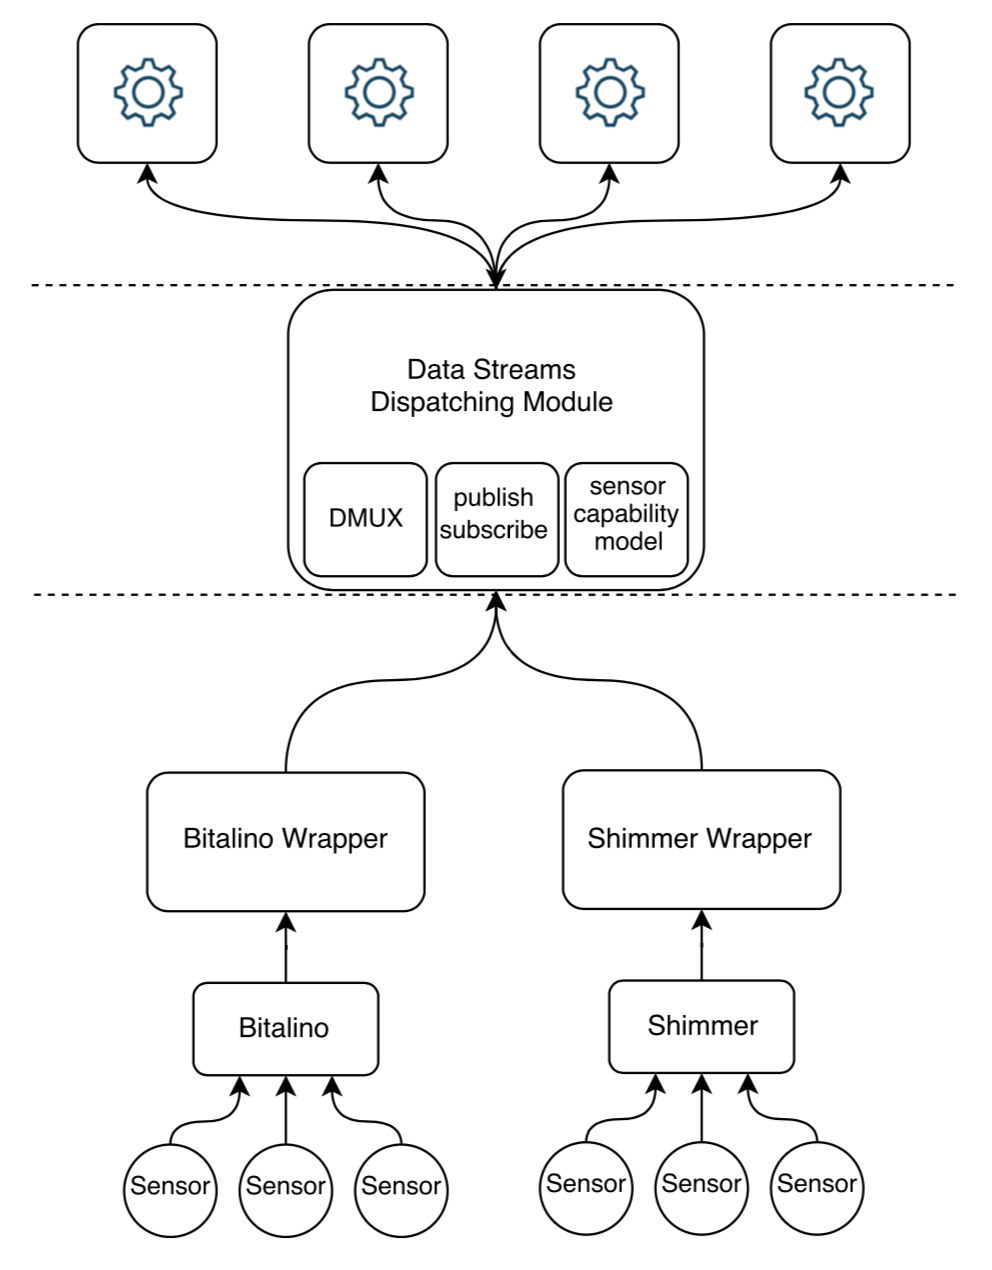
\includegraphics[width=0.65\textwidth]{images/demux.png}
    \caption{Sharing the collected data between multiple applications \cite{daniel}}
    \label{fig:demux}
\end{figure}

The combination of how these modules cooperate and communicate with each other affects the modularity and performance of the architecture. In the thesis, there are various proposed solutions. The naive solution was to fit all of the elements into each respective sensor wrapper, thus, prioritizing the performance and low resource usage, but making it impossible to distinguish data type from two sensor wrapper with the same data type. This is optimal for the cases where collection only occurs on one sensor board. An improved solution includes to place the demux between the application part and the wrapper layer and to insert the remaining elements in the respective application part. This solution resolves the overload of sensor wrappers performing other tasks besides collecting data; thus, the wrappers are untouched, and they send the data to the demux. However, there are several issues with this solution, e.g., due to various obstacles such as (1) every application module has to configure its sensor-capability model; (2) filter requested data packets from all the channels; (3) and deal with the collection speed on its own.

Addressing these issues leads to the final architecture, which is presented in Figure \ref{fig:demux}, and meets the demands identified in the requirements. In this solution, all elements are placed between the application part and the wrapper layer, forming the data stream dispatching module. The sensor wrapper connects directly to the data streams dispatching module; the module discovers all installed wrappers and populates the sensor-capability model with the data types from all installed sensors. By this, all applications can access a shared sensor-capability mode. A publish-subscribe mechanism enables application modules to subscribe to any capabilities with a preferred sampling rate. Correspondingly, an application module can publish data to other applications through the same interface. The demultiplexing element creates for each subscriber a copy of the data packet. 

To summarize, these three elements together establish \textit{the data stream dispatching module}. The final architecture has a couple of advantages, such as it is exceedingly extensible due to its maintainability. For instance, all communication with other layers occurs through one interface; this way, new instances can be added at any time, without the need for modifying large parts of the system. The system is also efficient due to packets are immediately sent to the application on request (without any buffers), and packets are only sent to the application requesting them, resulting in less resource and power usage, and more battery life. This tool is an improvement to Gjøby's solutions due to these facts.
